% -*-coding: utf-8 -*-
% Держать в начале каждого файла!

\documentclass[a4paper, 12pt]{extarticle}
\usepackage{metod}

\MTDSetPhysSection{Механика}
\MTDSetTitle{Изучение второго закона Ньютона}
\MTDDesignator{М--3}
\MTDSetGrade{10}

\MTDSetAuthors{И.~Н.~Грачева, В.~И.~Гребенкин, А.~Е.~Иванов, И.~А.~Коротова,
Е.~И.~Красавина, А.~В.~Кравцов, Н.~С.~Кулеба, Б.~В.~Падалкин,
Г.~Ю.~Шевцова, Т.~С.~Цвецинская}

\MTDSetEditorsGenCase{И.~Н.~Грачевой, А.~Е.~Иванова, А.~В.~Кравцова}

\begin{document}

\MTDTitlePage
\MTDInfoPage

\setcounter{section}{3}

\subsection{Цель работы}
Целью работы является экспериментальная проверка основного уравнения динамики материальной точки.

\subsection{Основные теоретические сведения}

Понятие материальной точки "--- одно из важнейших понятий механики. Материальной точкой называют тело, формой и размерами которого в заданных условиях движения можно пренебречь.

Всякое реальное тело можно разбить на большое число частей, сколь угодно малых по сравнению с размерами самого тела.

Каждую такую часть можно рассматривать как материальную точку, а само тело "--- как систему материальных точек.

Второй закон Ньютона "--- основной закон динамики материальной точки. В соответствии с ним ускорение~$\vec{a}$, сообщаемое материальной точке, прямо пропорционально вызывающей его силе~$\vec{F}$ и обратно пропорционально массе материальной точки~$m$: %ИЗМ: "массе тела~$m$" -> "массе материальной точки~$m$"
\begin{equation}
\label{eq:m3-newton's-law-2}
\vec{a} = \frac{\vec{F}}{m}.
\end{equation}

Силой, действующей на тело (или приложенной к телу), называют физическую величину, являющуюся мерой механического воздействия на это тело со стороны другого тела. Мы можем рассматривать движение тела под действием других тел как движение тела под действием приложенных к нему сил.

Если на материальную точку одновременно действуют несколько сил, то каждая из них сообщает материальной точке ускорение, определяемое выражением~\eqref{eq:m3-newton's-law-2} для данной силы, а суммарное ускорение является геометрической суммой сообщаемых силами ускорений. При этом говорят, что на материальную точку действует результирующая сила (равнодействующая), равная геометрической сумме отдельных действующих сил. Приведенные выше рассуждения выражают принцип независимости действия сил.

Соотношение~\eqref{eq:m3-newton's-law-2} показывает, что тела обладают свойством инертности. Именно благодаря своей инертности тело приобретает при действии силы конечное ускорение, изменяя свою скорость не мгновенно, а постепенно. Мерой инертности тела является масса.

Классическая механика исходит из того подтвержденного повседневным опытом положения, что масса тела "--- величина постоянная. В специальной теории относительности показано, что в общем случае масса тела зависит от его скорости, но при скоростях тел, намного меньших скорости света, эта зависимость незначительна. Классическая механика как раз и рассматривает движение тел при малых по сравнению со скоростью света скоростях.

Масса системы материальных точек равна сумме масс всех материальных точек, входящих в систему. Это утверждение выражает свойство аддитивности массы.

\subsection{Описание экспериментальной установки}
Схема экспериментальной установки приведена на рис.~\ref{fig:m3-equipment}. Установка состоит из рельса~\emph{1}, тележки~\emph{2} с подвесными грузами~\emph{3}, датчиков <<Старт>>~\emph{4} и <<Стоп>>~\emph{5}, ограничителя~\emph{6}, троса~\emph{7}, тарелки~\emph{8} с грузами~\emph{9} и электронного секундомера~\emph{10}.

\begin{figure}[h]
\begin{center}
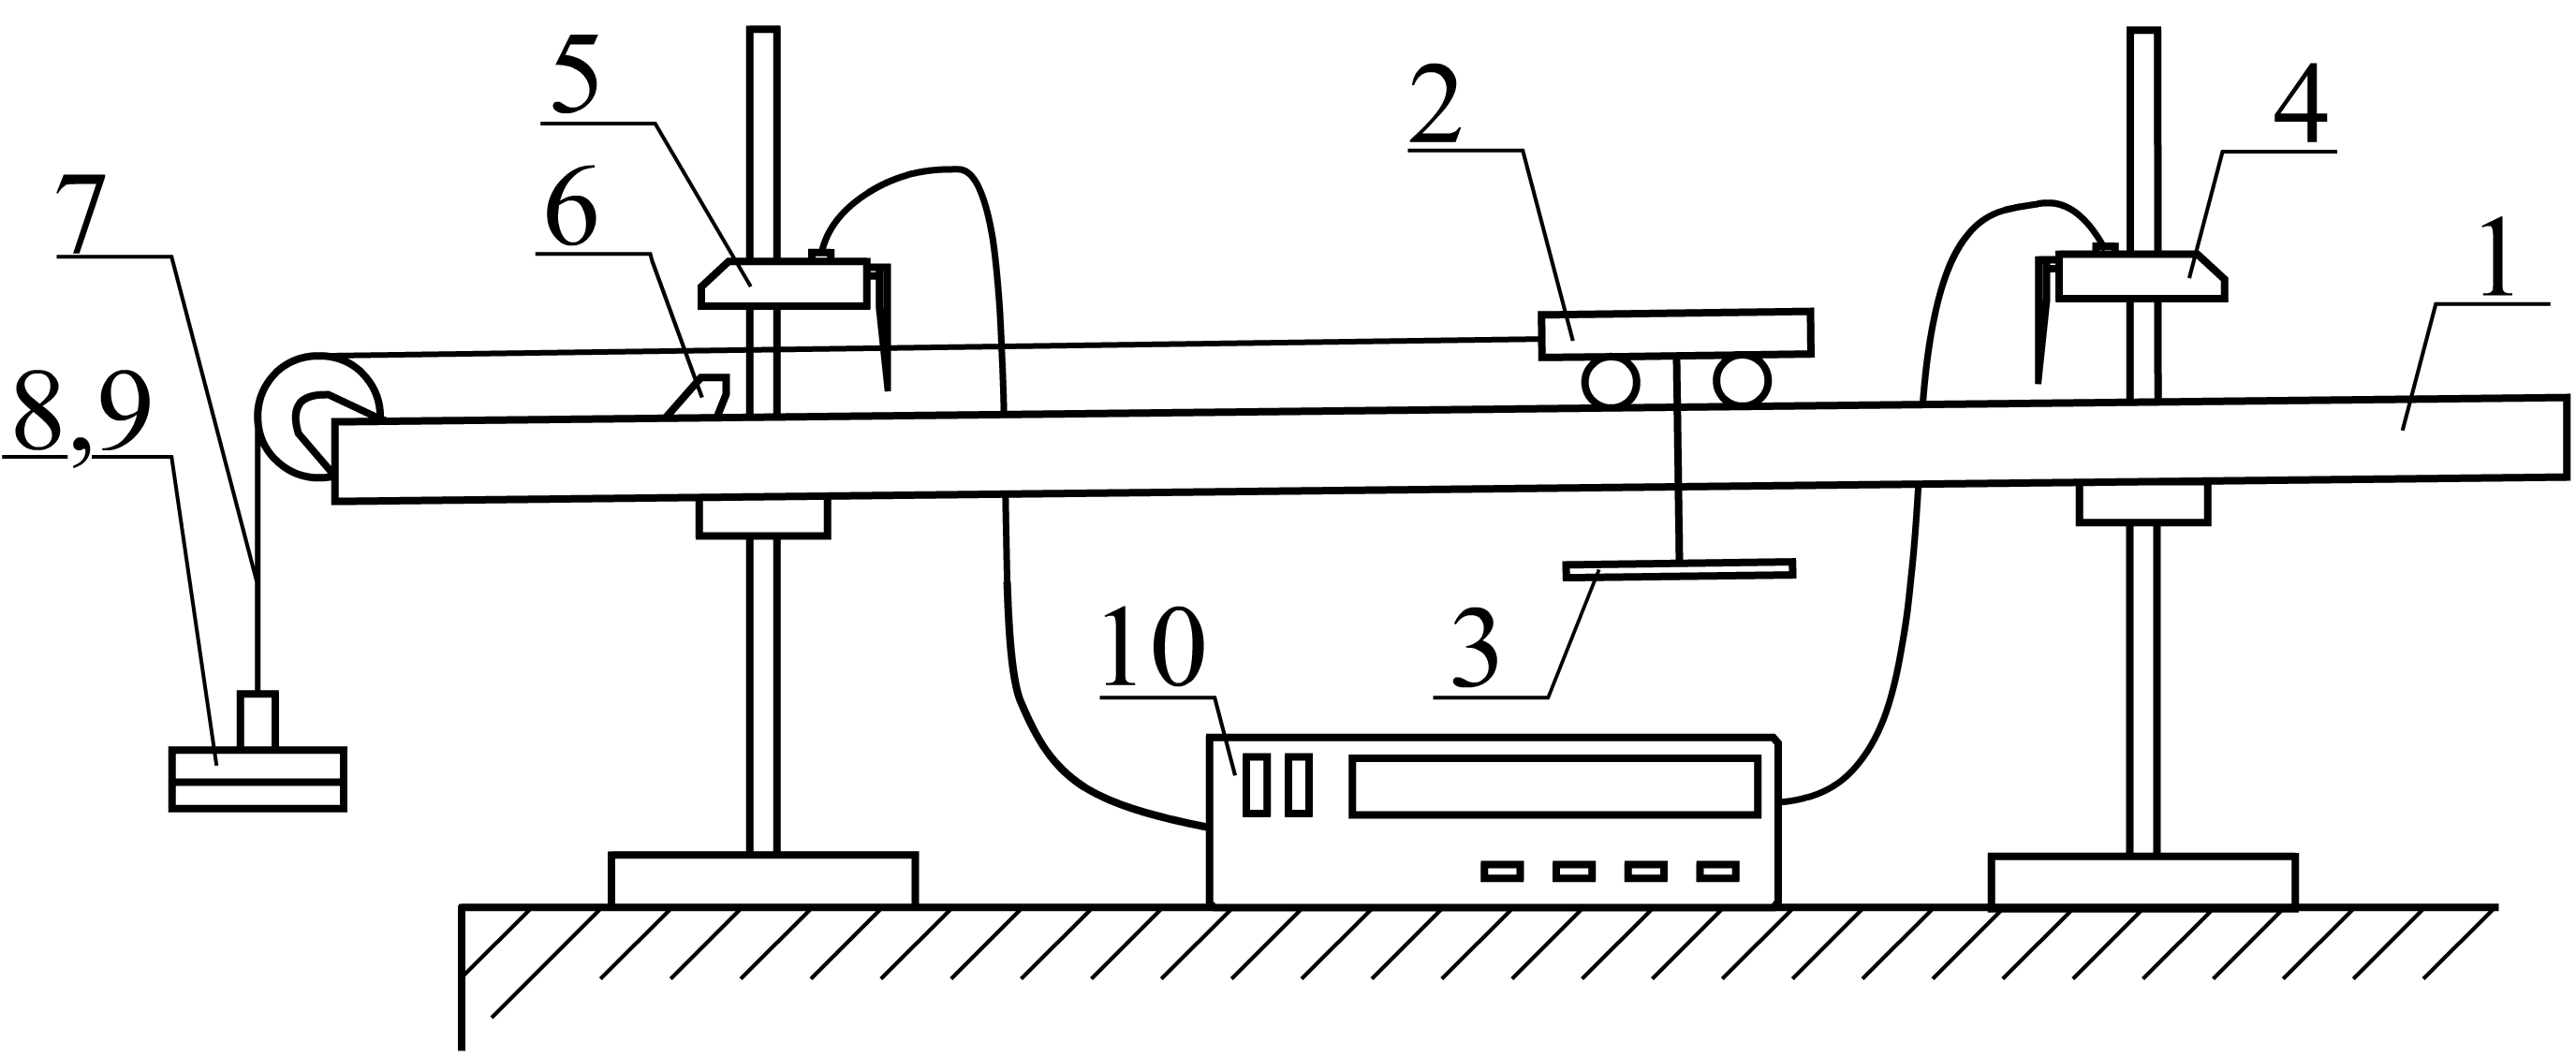
\includegraphics[scale = 0.14, keepaspectratio=true]{M3-RollerMachine}
\end{center}
\caption{Схема экспериментальной установки \label{fig:m3-equipment}}
\end{figure}

Сила тяжести, действующая на тарелку~\emph{8} с грузами~\emph{9}, создает ускорение системы <<тележка "--- трос "--- тарелка>>. Если тележка с этим ускорением движется с нулевой начальной скоростью от датчика <<Старт>>~\emph{4} до датчика <<Стоп>>~\emph{5}, то значение этого ускорения можно рассчитать из выражения %мб двоеточие?  | "тележка-трос-тарелка" какие здесь тире/дефисы?
\begin{equation}
\label{eq:m3-acceleration}
a = \frac{2s}{t^2}.
\end{equation}

Перемещение тележки с грузами измеряют линейкой, время движения "--- электронным секундомером~\emph{10}, запускаемым и останавливаемым автоматически с помощью датчиков~\emph{4}~и~\emph{5}. %ИЗМ: "запускаемого и останавливаемого" -> "запускаемым и останавливаемым"

В работе исследуются зависимости:
\begin{itemize}
\item ускорения от силы, действующей на систему, при постоянной массе системы
\item ускорения от массы системы при постоянной силе, действующей на систему. % точка в конце? скорее, да
\end{itemize}

Для компенсации силы трения, действующей со стороны рельса на тележку с грузами, рельс наклоняют под небольшим углом к горизонтальной плоскости. Значение угла наклона подбирается экспериментально.

\subsection{Порядок выполнения работы и обработки результатов измерений}
\MTDTask{Исследование зависимости ускорения от силы, действующей на систему, при постоянной массе системы}

%\underline{\textbf{Задание 1.}} \emph{Исследование зависимости ускорения от силы, действующей на систему, при постоянной массе системы.} %оставила все как было. хотелось бы автоматическую нумерацию и мб не подчеркивание, хотя и так вроде норм
\begin{enumerate}
\item В процессе домашней подготовки начертите в протоколе эксперимента таблицы~\ref{tab:m3-res-exp-1}, \ref{tab:m3-res-exp-2} и \ref{tab:m3-res-exp-3} для записи результатов измерений и вычислений. %с пунктами какая-то хрень: 2 первых. мб поменять "задание 1" и первый пункт местами? хотя тоже плохо будет; раз вывод во втором задании, значит таблицы будут в первом | "начертите" не самый прекрасный глагол, но прекраснее не могу придумать | ИЗМ: "Подготовьте"-> "В процессе домашней подготовки начертите"
%здесь было примечание

\begin{table}[h]
\caption{\label{tab:m3-res-exp-1}}
\begin{center}
\begin{tabular}{|c|>{\centering\arraybackslash} m{1.5cm}|}
\hline
Масса тарелки $M_1$,~\Units{кг} & 0,003 \\ \hline
Масса тележки $M_2$,~\Units{кг} & 0,242 \\ \hline
Общая масса системы $M$,~\Units{кг} (задание 1) & \\ \hline
Перемещение тележки $s$,~\Units{м} & \\ \hline
Сила, действующая на систему, $F$,~\Units{мН} (задание 2) & \\ \hline  %мб Сила F, действующая на систему,? или так нельзя наверное
\end{tabular}
\end{center}
\end{table}

\begin{table}[h] %в моей тетради всего 3 измерения, но не буду менять
\caption{\label{tab:m3-res-exp-2}}
\begin{center}
\begin{tabular}{|>{\centering\arraybackslash} m{2.0cm}|>{\centering\arraybackslash} m{2.0cm}|>{\centering\arraybackslash} m{2.0cm}|>{\centering\arraybackslash} m{2.0cm}|>{\centering\arraybackslash} m{2.0cm}|>{\centering\arraybackslash} m{2.0cm}|} %возможно, ширина должна быть другой, зато 2 таблицы одинаковой ширины, хотя возможно надо верхнюю увеличить | черт, вторая таблица переехала к первой, теперь они разной ширины и на одной странице, но растягивать первую - садизм, вторую можно, конечно, немного сузить, но зачем?
\hline
Номер измерения & Масса грузов на тарелке $m_1$,~\Units{кг} & Масса грузов на тележке $m_2$,~\Units{кг} & Время движения $t$,~\Units{с} & Ускорение $a$,~$\Units{\text{м}/\text{с}^2$} & Сила $F$,~\Units{мН} \\ \hline %ИЗМ: \textnumero -> "Номер"
1 & & & & & \\ \hline
2 & & & & & \\ \hline
3 & & & & & \\ \hline
4 & & & & & \\ \hline
\end{tabular}
\end{center}
\end{table}

\begin{table}[h]
\caption{\label{tab:m3-res-exp-3}}
\begin{center}
\begin{tabular}{|>{\centering\arraybackslash} m{2.0cm}|>{\centering\arraybackslash} m{2.0cm}|>{\centering\arraybackslash} m{2.0cm}|>{\centering\arraybackslash} m{2.0cm}|>{\centering\arraybackslash} m{2.0cm}|>{\centering\arraybackslash} m{2.0cm}|}
\hline
Номер измерения & Масса грузов на тележке $m_2$,~\Units{кг} & Время движения $t$,~\Units{с} & Ускорение $a$,~$\Units{\text{м}/\text{с}^2$} & Масса системы $M$,~\Units{кг} & $F/M(a)$, $\Units{\text{м}/\text{с}^2}$ \\ \hline % F/M(a): что здесь a? указание на то, что M зависит от a или что получится? опять же, нужен ли \frac | %ИЗМ: \textnumero -> "Номер"
1 & 0 & & & & \\ \hline
2 & 0,120 & & & & \\ \hline
3 & 0,240 & & & & \\ \hline
\end{tabular}
\end{center}
\end{table}

\item Ознакомьтесь с устройством экспериментальной установки и получите у преподавателя допуск к работе.
\item Для компенсации силы трения положите на тележку грузы общей массой 0,126~\Units{кг} и наклоните рельс настолько, чтобы тележка двигалась равномерно.
\item Измерьте линейкой расстояние между датчиками <<Старт>> и <<Стоп>>, результат запишите в таблицу~\ref{tab:m3-res-exp-1}.
\item Прикрепите к тележке нить с тарелкой и одним грузом массой 3~\Units{г}. Перебросьте нить через блок. Рассчитайте общую массу системы и запишите результат в таблицу~\ref{tab:m3-res-exp-1}.
\item Рассчитайте по приведенному ниже выражению~\eqref{eq:m3-force} силу $F$, действующую на систему, результат расчета запишите в таблицу~\ref{tab:m3-res-exp-2}.
\begin{equation}
\label{eq:m3-force}
F = (M_1 + m_1)g.
\end{equation}
\item Резким, но не сильным ударом по крючку датчика <<Старт>> пустите тележку. При этом происходит пуск секундомера. В момент прохождения тележки мимо датчика <<Стоп>> происходит остановка секундомера. Запишите показание секундомера в таблицу~\ref{tab:m3-res-exp-2}.
\item Пользуясь выражением~\eqref{eq:m3-acceleration}, рассчитайте ускорение и запишите результат в таблицу~\ref{tab:m3-res-exp-2}.
\item Переложите с тележки на тарелку один груз массой 3~\Units{г}.
\item Повторите операции пп.~6--9 несколько раз, пока все малые грузы не будут переложены с тележки на тарелку.
\item На миллиметровой бумаге постройте график зависимости ускорения $a$ от силы $F$ при постоянной массе $M$.
\end{enumerate}

\MTDTask{Исследование зависимости ускорения от массы движущегося тела при постоянной силе, действующей на систему}

%\underline{\textbf{Задание 2.}} \emph{Исследование зависимости ускорения от массы движущегося тела при постоянной силе, действующей на систему.}
\begin{enumerate}
\item Снимите с тележки все грузы, на тарелку положите два груза массой по 3~\Units{г} каждый. По выражению~\eqref{eq:m3-force} рассчитайте силу, действующую на систему, результат занесите в таблицу~\ref{tab:m3-res-exp-1}.
\item Определите ускорение тележки, повторив операции п.~7 задания~1 и пользуясь выражением~\eqref{eq:m3-acceleration}. Результат запишите в таблицу~\ref{tab:m3-res-exp-3}.
\item Положите на тележку груз массой 120~\Units{г} и повторите п.~2.
\item Повторите п.~3 еще один раз.
\item Рассчитайте по полученным данным отношения силы к массе движущихся тел $F/M$, результаты запишите в таблицу~\ref{tab:m3-res-exp-3}. Постройте график зависимости ускорения от массы системы при постоянной силе, действующей на систему. %мб \dfrac, мб просто F/M
\item По результатам выполнения заданий~1~и~2 сформулируйте выводы и напишите заключение к работе.
\end{enumerate}

\subsection{Контрольные вопросы}
\begin{enumerate}
\item Что является причиной ускорения? Как направлено ускорение?
\item Что можно сказать об ускорениях двух взаимодействующих тел?
\item Почему нагруженный автомобиль на булыжной мостовой движется более плавно, чем этот же автомобиль без груза?
\item В чем состоит свойство, называемое инертностью тела?
\item Как сравнить массы двух тел в условиях невесомости?
\item Дайте определение понятию <<сила>>.
\item Может ли тело, на которое действуют силы, двигаться без ускорения?
\item Сформулируйте второй закон Ньютона.
\item Верны ли следующие утверждения:
	\begin{itemize}
	\item <<Скорость тела определяется действующей на него силой>>
	\item <<Тело движется туда, куда направлена действующая на него сила>>?
	\end{itemize}
\item Два шара, соединенные невесомой нерастяжимой нитью, лежат на гладкой горизонтальной плоскости. У правого шара масса больше. Одинаковая по модулю сила действует сначала на правый шар вправо, затем на левый шар влево. Одинаково ли натяжение нити в этих случаях?
\item Какую силу называют силой тяжести; весом?
\item Масса каких тел, используемых в данной работе, не учитывается при проведении расчетов? Как это влияет на результаты работы?
\item Каким образом в работе компенсируется влияние трения?
\item Какая внешняя сила действует на систему тел в работе? Почему в ходе каждого опыта ее можно считать постоянной?
\item Второй закон Ньютона выполняется для материальных точек. Однако тела, используемые в работе, таковыми не являются. Какие допущения позволяют нам считать результаты работы подтверждением второго закона Ньютона? %ИЗМ: "Тела, используемые" -> "Однако тела, используемые"
\end{enumerate}


\end{document}
